\documentclass{standalone}
% \documentclass{article}

\usepackage{tikz}
\usetikzlibrary{calc}

\begin{document}

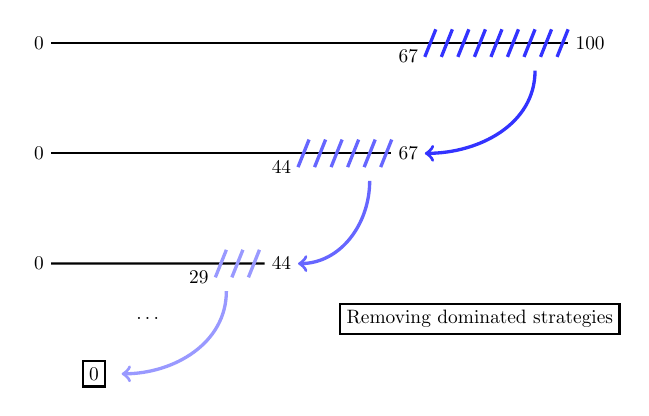
\begin{tikzpicture}[thick,scale=0.7, every node/.style={scale=0.7}]
    % First level of play
    \node (0) at (0,0) {$0$};
    \node (100) at (10,0) {$100$};
    \draw [thick] (0) -- (100);
    \node [below] at (6.7,0) {$67$};

    % Getting rid of dominated strategies
    \foreach \x in {7, 7.3, 7.6, 7.9, 8.2, 8.5, 8.8, 9.1, 9.4}
    {
        \draw [blue!80, very thick] (\x,-.25) -- (\x + .2,.25);
    }
    \draw [very thick, blue!80] (9, -.5) edge[out=270,in=0,->] (7, -2);

        % Second level of play
        \node (0) at (0,-2) {$0$};
        \node (67) at (6.7,-2) {$67$};
        \draw [thick] (0) -- (67);
        \node [below] at (4.4,-2) {$44$};

        % Getting rid of dominated strategies
        \foreach \x in {4.7, 5, 5.3, 5.6, 5.9, 6.2}
        {
            \draw [blue!60, very thick] (\x,-2.25) -- (\x + .2,-1.75);
        }
        \draw [very thick, blue!60] (6, -2.5) edge[out=270,in=0,->] (4.7, -4);

            % Third level of play
            \node (0) at (0,-4) {$0$};
            \node (44) at (4.4,-4) {$44$};
            \draw [thick] (0) -- (44);
            \node [below] at (2.9,-4) {$29$};

            % Getting rid of dominated strategies
            \foreach \x in {3.2, 3.5, 3.8}
            {
                \draw [blue!40, very thick] (\x,-4.25) -- (\x + .2,-3.75);
            }

                % Final level of play
                \node at (2, -5) {\dots};
                \node (0) at (1,-6) [draw] {$0$};
                \draw [very thick, blue!40] (3.4, -4.5) edge[out=270,in=0,->] (1.5, -6);

    \node at (8, -5) [draw] {Removing dominated strategies};
\end{tikzpicture}

\end{document}
